% Copyright 2004 by Till Tantau <tantau@users.sourceforge.net>.
%
% In principle, this file can be redistributed and/or modified under
% the terms of the GNU Public License, version 2.
%
% However, this file is supposed to be a template to be modified
% for your own needs. For this reason, if you use this file as a
% template and not specifically distribute it as part of a another
% package/program, I grant the extra permission to freely copy and
% modify this file as you see fit and even to delete this copyright
% notice. 

\documentclass{beamer}
% Replace the \documentclass declaration above
% with the following two lines to typeset your 
% lecture notes as a handout:
%\documentclass{article}
%\usepackage{beamerarticle}

\usepackage{graphicx}
\usepackage[utf8]{inputenc}
 
\graphicspath{ {img/} }


% There are many different themes available for Beamer. A comprehensive
% list with examples is given here:
% http://deic.uab.es/~iblanes/beamer_gallery/index_by_theme.html
% You can uncomment the themes below if you would like to use a different
% one:
%\usetheme{AnnArbor}
%\usetheme{Antibes}
%\usetheme{Bergen}
%\usetheme{Berkeley}
%\usetheme{Berlin}
%\usetheme{Boadilla}
%\usetheme{boxes}
%\usetheme{CambridgeUS}
%\usetheme{Copenhagen}
%\usetheme{Darmstadt}
%\usetheme{default}
%\usetheme{Frankfurt}
%\usetheme{Goettingen}
%\usetheme{Hannover}
%\usetheme{Ilmenau}
%\usetheme{JuanLesPins}
%\usetheme{Luebeck}
%\usetheme{Madrid}
%\usetheme{Malmoe}
%\usetheme{Marburg}
%\usetheme{Montpellier}
%\usetheme{PaloAlto}
%\usetheme{Pittsburgh}
%\usetheme{Rochester}
%\usetheme{Singapore}
%\usetheme{Szeged}
\usetheme{Warsaw}

\title{Programming with Python}

% A subtitle is optional and this may be deleted
\subtitle{Lesson 1: Setting up and basics}

%\author{F.~Author\inst{1} \and S.~Another\inst{2}}
% - Give the names in the same order as the appear in the paper.
% - Use the \inst{?} command only if the authors have different
%   affiliation.

%\institute[Universities of Somewhere and Elsewhere] % (optional, but mostly needed)
%{
%  \inst{1}%
%  Department of Computer Science\\
%  University of Somewhere
%  \and
%  \inst{2}%
%  Department of Theoretical Philosophy\\
%  University of Elsewhere}
% - Use the \inst command only if there are several affiliations.
% - Keep it simple, no one is interested in your street address.

\date{November 1st, 2016}
% - Either use conference name or its abbreviation.
% - Not really informative to the audience, more for people (including
%   yourself) who are reading the slides online

\subject{Python Lessons}
% This is only inserted into the PDF information catalog. Can be left
% out. 

% If you have a file called "university-logo-filename.xxx", where xxx
% is a graphic format that can be processed by latex or pdflatex,
% resp., then you can add a logo as follows:

% \pgfdeclareimage[height=0.5cm]{university-logo}{university-logo-filename}
% \logo{\pgfuseimage{university-logo}}

% Delete this, if you do not want the table of contents to pop up at
% the beginning of each subsection:
%\AtBeginSubsection[]
%{
%  \begin{frame}<beamer>{Outline}
%    \tableofcontents[currentsection,currentsubsection]
%  \end{frame}
%}

% Let's get started
\begin{document}

\begin{frame}
  \titlepage
\end{frame}

%\begin{frame}{Outline}
%  \tableofcontents
%  % You might wish to add the option [pausesections]
%\end{frame}

% Section and subsections will appear in the presentation overview
% and table of contents.
\section{Introduction}

\subsection{Setting up and basics}

\begin{frame}{What is Python? What is programming?}
\begin{figure}[h]
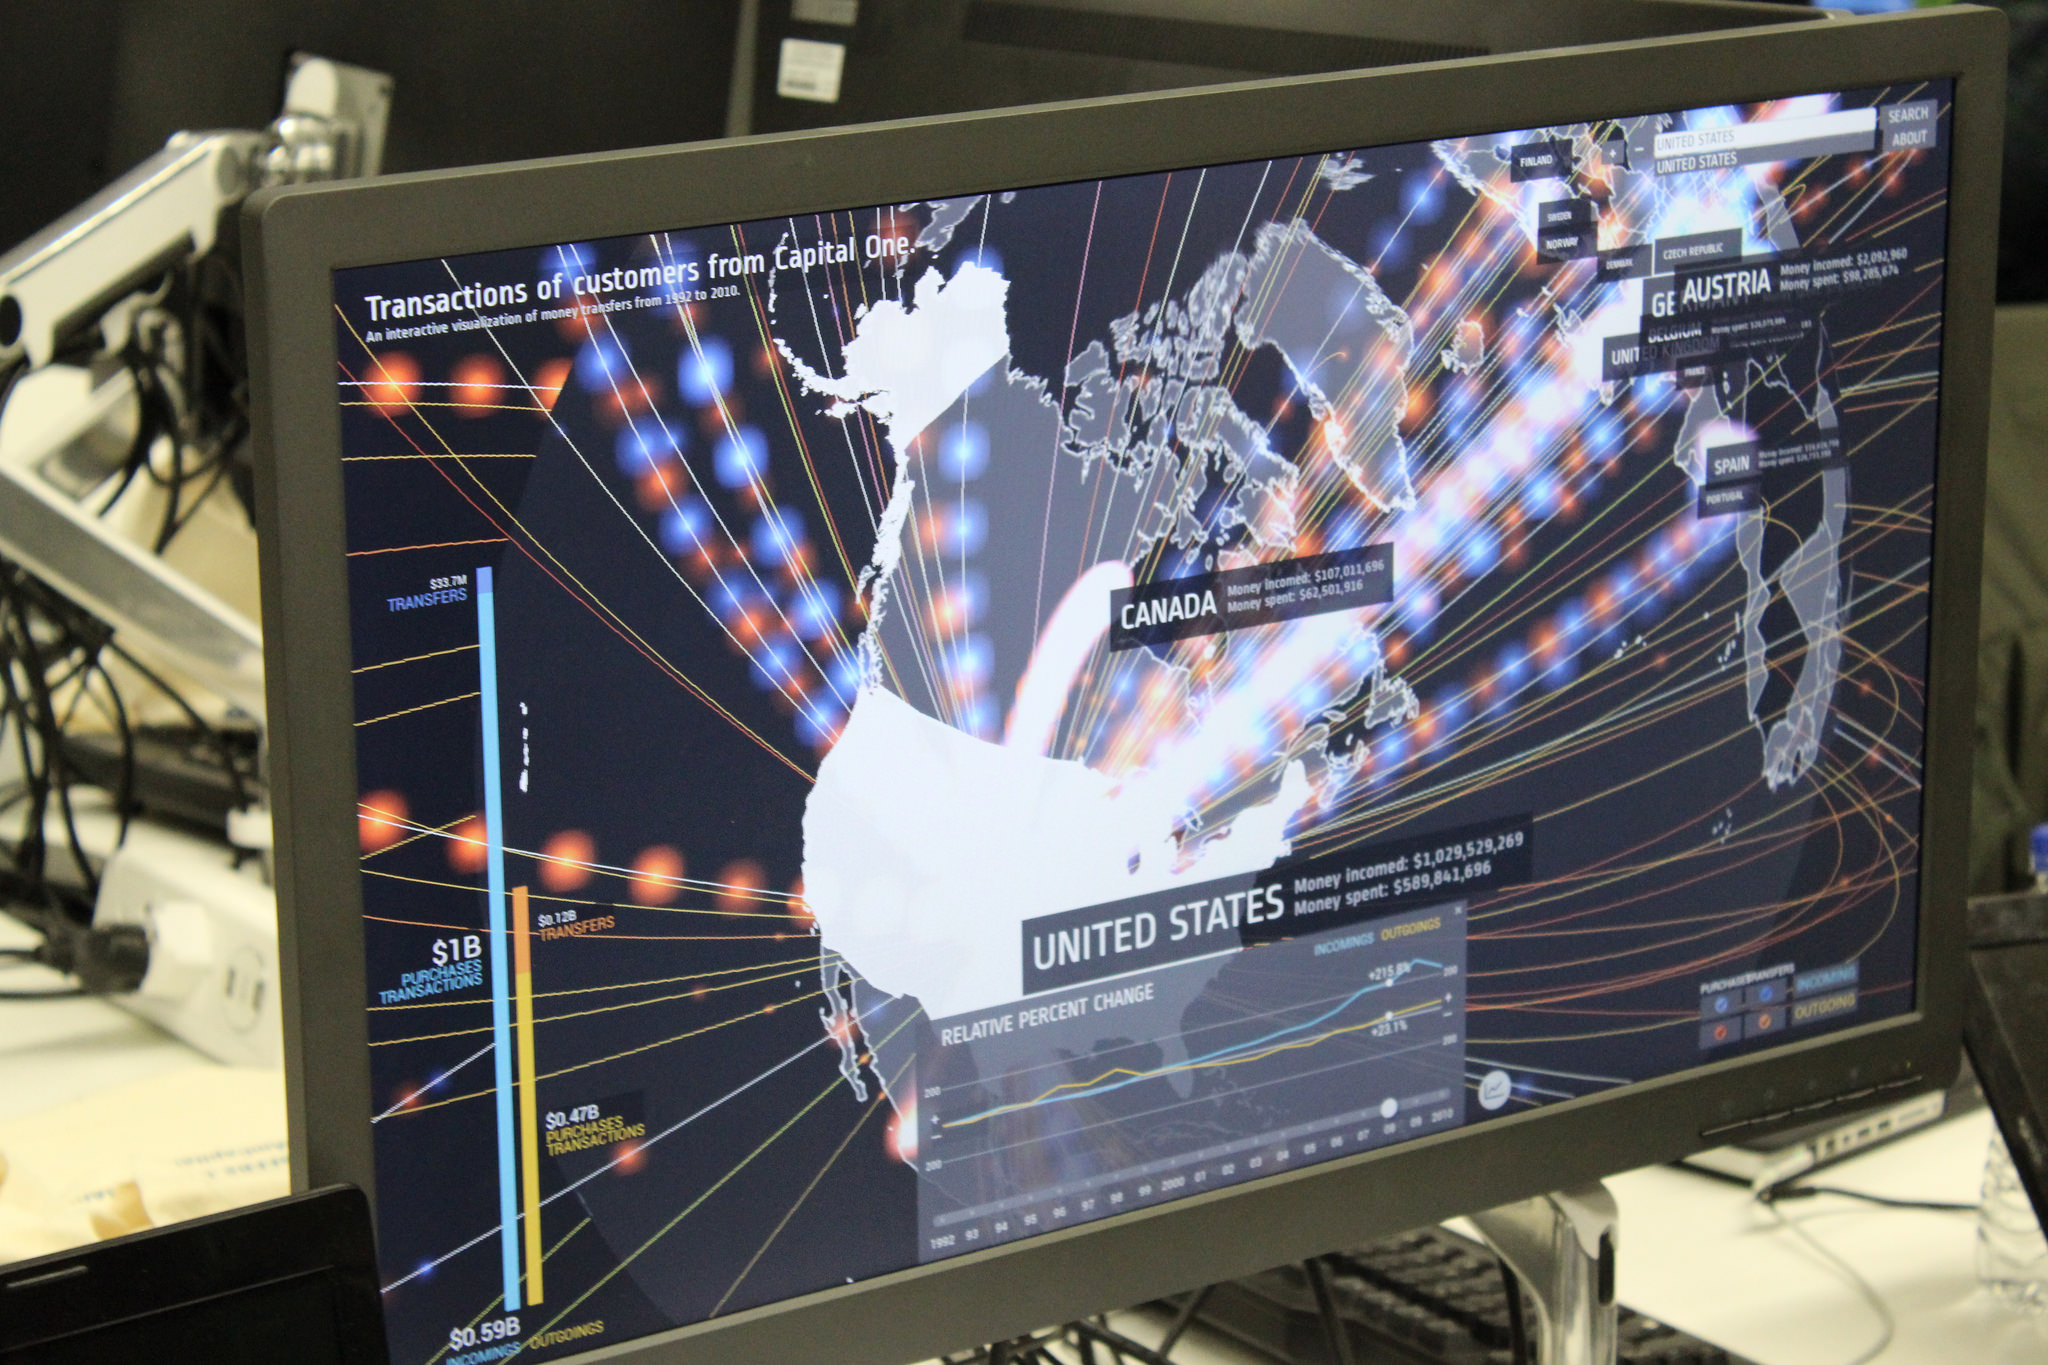
\includegraphics[width=0.7\textwidth]{wow}
\caption{Image curtosy of HackSocNotts}
\end{figure}
\end{frame}

\begin{frame}{Making a cup of tea}

How do you make a cup of tea?
\pause
\begin{enumerate}

  \item {
    Boil the kettle.
    \pause % The slide will pause after showing the first item
  }
  \item {   
    Get a mug and a teabag.
    \pause
  }
  % You can also specify when the content should appear
  % by using <n->:
  \item {
    Put a teabag in the mug.
    \pause
  }
  \item {
    Stir and wait.
    \pause
  }
  % or you can use the \uncover command to reveal general
  % content (not just \items):
  \item {
    Enjoy!
  }
  \end{enumerate}

\end{frame}


% You can reveal the parts of a slide one at a time
% with the \pause command:
\begin{frame}{Making a cup of tea}

Computers need a little more help...
\pause
\begin{enumerate}

  \item {
    GET Water.
    \pause % The slide will pause after showing the first item
  }
  \item {
    GET Kettle.
    \pause % The slide will pause after showing the first item
  }
  \item {   
    ADD Water to Kettle.
    \pause
  }
  % You can also specify when the content should appear
  % by using <n->:
  \item {
    SWITCH ON Kettle.
    \pause
  }
  \item {
    SLEEP until Kettle finished.
    \pause
  }
  
  \item {
    GET Mug.
    \pause
  }

  \item {
    Etc...
  }

  \end{enumerate}

\end{frame}


\section{About Python}

\begin{frame}{What is Python?}

\begin{itemize}

  \item {
    A procedural, interpreted scripting language.
    \pause % The slide will pause after showing the first item
  }
  \item {
    Two major versions: 2.7 (2010) \& 3.x (Currently at 3.5 as of 2015).
    \pause % The slide will pause after showing the first item
  }
  \item {   
    We will be using the \textit{pycharm} IDE to write our python code. 
  }

  \end{itemize}

\end{frame}

\section{Installing Python \& PyCharm}

\begin{frame}{Installing the Python 3.5.2 interpreter}
\begin{itemize}
  \item {
    Windows: \textbf{https://www.python.org/downloads/windows/}
  }
  \item {
    Mac OSX: \textbf{https://www.python.org/downloads/mac-osx/}
  }
  \item {
    Linux: Either \textbf{sudo apt-get install python3} or \textbf{https://www.python.org/downloads/source/}
  }
\end{itemize}

If at any time you get stuck, just stick your hand up and we'll come help.

\end{frame}

\begin{frame}{Installing PyCharm}
\textbf{https://www.jetbrains.com/pycharm/download/}
\end{frame}

% Placing a * after \section means it will not show in the
% outline or table of contents.
\section*{Our First Program}

\begin{frame}{Keywords}
Before we begin, below are a couple of keywords used quite often when programming:
\begin{itemize}
  \item[] Syntax - How Python understands your code. Kind of like the grammar of your code.
  \item[] Console - Where text is printed to and where you can input text.
  \item[] Interpreter - The thing Python uses to understand your code.
  \item[] Operator - Things like plus, minus, multiply and divide. They do things.
\end{itemize}
\end{frame}

\begin{frame}{Hello World!}
Now that we have all prerequisites installed, load up PyCharm and start a new project.\\ \pause
We are going to build a simple program which prints the words "Hello, World!".
\end{frame}

\begin{frame}
The \textit{print} command prints something to the console:
\begin{figure}[h]
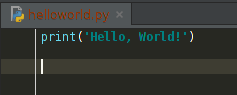
\includegraphics[width=0.7\textwidth]{helloworld}
\end{figure}
\end{frame}

\begin{frame}
Now that we have our code, we want to execute it. This can be done by hitting the green arrow in the top right corner.
\begin{figure}[h]
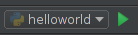
\includegraphics[width=0.7\textwidth]{arrow}
\end{figure}

Feel free to change the code inside the print to print whatever message you want!
\end{frame}

\begin{frame}{Reading in input}
A program that just prints a string is pretty rubbish. What'd be great would be if we could tell it what to print.\\
\pause
The \textit{input} command allows us to input what we want into the program. However, we need somewhere to put our input, before we can display it.
\end{frame}

\begin{frame}
Now our program can display our name:
\begin{figure}[h]
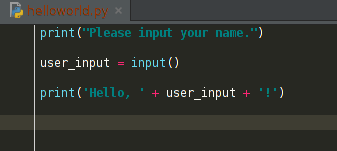
\includegraphics[width=0.7\textwidth]{input}
\end{figure}
\pause
What have we actually done here?
\end{frame}

\begin{frame}{Variables}
Variables are a container for things. They can change when you want them to and have any name you want.\\
\pause
In the previous example we specified a new variable called \textit{name} where we stored the value we wanted to input.\\
\pause
Variables can be many different things including:
\pause
\begin{itemize}
  \item An integer (1,2,3 etc) \pause
  \item A character ('a','b','c' etc) \pause
  \item A string ("Hello, World!", "I love python xo" etc) \pause
  \item A float (1.45345, 24.4562389, 7.4234 etc) \pause
  \item An array ([1,2,7,4,7], ['p', 'y', 't', 'h', 'o', 'n'] etc) \pause
  \item Or more!
\end{itemize}
\pause
Some of these types can do things others can't. For example, we can subtract an integer from another, but we can't subtract a string from another.
\end{frame}

\begin{frame}{A simple adding calculator}
Using these variable types, we can convert our input into a different type! To convert a variable into a different type, we wrap the variable in the type we want to convert it to.
\pause
\begin{figure}[h]
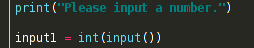
\includegraphics[width=0.7\textwidth]{calc1}
\end{figure}
\pause
Here, the input we are asking for is being turned into an integer. Another name for this is we are \textbf{casting} the input to an integer.\\
Q: What happens if you put in something other than a number?
\end{frame}


\begin{frame}{Our lovely calculator}
Building on from that, we can combine what we have talked about to make a very simple calculator, which asks for two numbers, adds them together (using the \textit{+} operator), and then outputs them to the user.
\pause
\begin{figure}[h]
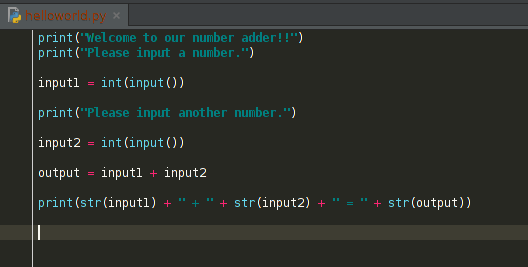
\includegraphics[width=0.7\textwidth]{calc}
\end{figure}
\pause
Note we had to \textbf{cast} our integer variables to strings using \textit{str()} for \textit{print} to work.
\end{frame}

\begin{frame}{That's all for tonight!}
  To summarise:
  \begin{itemize}
  \item We have installed Python and PyCharm
  \item We have learnt about variables and variable types
  \item We have learnt about printing and asking for input from the user
  \item We have made a sweet ass calculator!
  \end{itemize}
\end{frame}

\begin{frame}{For next week}
Source code plus lecture slides will be available online soon after the lesson.\\
If you are new to HackSocNotts, please join us on \textit{http://hacksocnotts.slack.com}.\\
If you have any questions, feel free to ask now or over slack.\\
\end{frame}

\end{document}


